\documentclass[12pt, a4paper]{article}
\usepackage[vietnamese]{babel}
\usepackage[utf8]{inputenc}
% \usepackage{xeCJK}
\usepackage{graphicx,wrapfig,lipsum}
\usepackage{mathtools}
\usepackage{natbib}
\usepackage{hyperref}
\usepackage{graphicx}
\usepackage{verbatim}
\usepackage{amsmath}
\usepackage{minted}
\usepackage{graphicx}
\usepackage{array}
\usepackage[colorinlistoftodos]{todonotes}
\usepackage{listings}
\usepackage{hyperref}
\hypersetup{
    colorlinks=true,
    linkcolor=blue,
    filecolor=magenta,      
    urlcolor=cyan,
}

\usepackage{indentfirst}
\usepackage{listings}
\usepackage{xcolor}
\usepackage{indentfirst}

\definecolor{codegreen}{rgb}{0,0.6,0}
\definecolor{codegray}{rgb}{0.5,0.5,0.5}
\definecolor{codepurple}{rgb}{0.58,0,0.82}
\definecolor{backcolour}{rgb}{0.95,0.95,0.92}


\begin{document}
\begin{titlepage}

\newcommand{\HRule}{\rule{\linewidth}{0.5mm}} 

\center % Căn lề giữa
 
%----------------------------------------------------------------------------------------
%	HEADING 
%----------------------------------------------------------------------------------------

% Tên trường
\textsc{\LARGE Đại học quốc gia TP.HCM}
\newline
\textsc{\LARGE Trường đại học công nghệ thông tin}\\[1.5cm] 

% Logo trường

\graphicspath{ {./logo/} }
 

\includegraphics[scale=0.5]{logo-uit.png}\\[1.5cm]

% Chuyên ngành 
\textsc{\Large Ngành KHMT}\\[0.5cm] 

% Môn học
\textsc{\large Môn học: CS115.N11.KHTN }\\[1.0cm] 

%----------------------------------------------------------------------------------------
%	TITLE 
%----------------------------------------------------------------------------------------

\HRule \\[0.4cm]
{ \huge \bfseries Tiêu đề: Decision Tree}\\[0.4cm] 
\HRule \\[1.5cm]
 
%----------------------------------------------------------------------------------------
%	TÁC GIẢ 
%----------------------------------------------------------------------------------------

\begin{minipage}{0.4\textwidth}
\begin{flushleft} \large
\emph{Sinh viên:}\\
Lương Toàn Bách \\
- 21521845 -
\end{flushleft}
\end{minipage}
~
\begin{minipage}{0.4\textwidth}
\begin{flushright} \large
\emph{Giảng viên:} \\
Lương Ngọc Hoàng
\end{flushright}
\end{minipage}\\[2cm]


%----------------------------------------------------------------------------------------
%	NỘI DUNG 
%----------------------------------------------------------------------------------------



\vfill 

\end{titlepage}
\tableofcontents
\newpage
\section{CÁC KHÁI NIỆM CƠ BẢN}
\subsection{Giới thiệu}
Decision Tree là một kiểu mô hình dự đoán thuộc loại supervised learning không có tham số đầu vào có cấu trúc biểu diễn dươi dạng cây.\\
\begin{wrapfigure}{l}[0pt]{0.625\linewidth}
    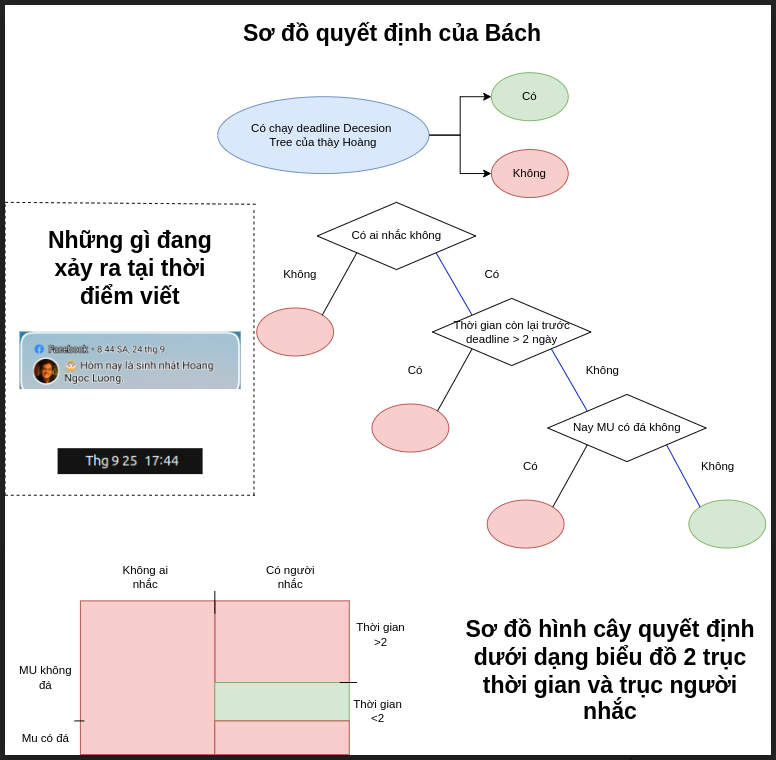
\includegraphics[scale=0.3]{Decesion_Tree_Graph.png}
    \caption{Minh hoạ cây quyết định trong đời sống}
\end{wrapfigure}
Dùng để giải quyết các bài toán bằng cách chia dữ liệu thành các tập khác nhau .Với mỗi phép chia liên tiếp, các tập con thu được trong tập kết quả sẽ ngày càng giống nhau.và mỗi tập sẽ chỉ có 1 kết quả output ứng với nó. \\


Mục tiêu xây dựng một Decision Tree là tạo ra một mô hình dự đoán giá trị của một biến mục tiêu bằng các quy tắc quyết định học từ các thuộc tính dữ liệu (data features) trên tập dữ liệu huấn luyện (training set). 
\subsection{Phân loại}
Có 2 loại cây quyết định từng loại cây quyết định ước lượng các hàm có giá trị khác nhau là:

\begin{itemize}
    \item Cây hồi quy(Regression Tree): số thực.
    \item Cây phân loại(Classification Tree): giá trị rời rạc(class). \\
\end{itemize}

\section{DECESION TREE TRONG SKLEARN}
\subsection{Những thứ thư viện cung cấp}
Thư viện cung cấp cho người dùng 2 modulo để xử lý 2 loại Decesion Tree đã nói ở trên:
\begin{itemize}
    \item sklearn.tree.DecisionTreeClassifier cho phân loại.
    \item sklearn.tree.DecisionTreeRegressor cho hồi quy.
\end{itemize}
\subsection{Cách sử dụng}
Vì cách sử dụng của hai module gần giống nhau nên bản báo cáo này sẽ chỉ nói về cách sử dụng của 
Decesion-TreeClassifier.\\ \\
Code demo trên bộ dữ liệu iris được trình bày tại \href{https://colab.research.google.com/drive/11R9PA-roN8-FNO-1D62fZ2f7JaTlvQk5#scrollTo=FOGFfr1hM1a1}{đây} được tham khảo tại trang \href{https://scikit-learn.org/stable/modules/generated/sklearn.tree.DecisionTreeRegressor.html}{sklearn}.

\subsubsection{Import thư viện}
\begin{minted}
[
frame=lines,
framesep=2mm,
baselinestretch=1.2,
fontsize=\footnotesize,
linenos
]
{python}
from sklearn import tree
from sklearn.tree import DecisionTreeClassifier

\end{minted}

\subsubsection{Huẩn luyện mô hình}
\begin{minted}
[
frame=lines,
framesep=2mm,
baselinestretch=1.2,
fontsize=\footnotesize,
linenos
]
{python}
# Tạo 1 instance của Decesion Tree
model = DecisionTreeClassifier(criterion = "entropy", min_samples_split = 3, max_depth = 10, max_leaf_nodes = 20)
# Huấn luyện the cây vói training set (X_train, y_train) 
# Với X là ma trận inputs of và y is ma trận cột các kết quả(labels)
model.fit(X_train, y_train)
\end{minted}

\subsubsection{Dự đoán kết quả thông qua mô hình đã huấn luyện}
\begin{minted}
[
frame=lines,
framesep=2mm,
baselinestretch=1.2,
fontsize=\footnotesize,
linenos
]
{python}
predicted = model.predict(X_test)
\end{minted}

\subsubsection{Các tham số đầu vào của Decesion Tree}
\begin{itemize}
    \item creterion\begin{itemize}
        \item Chọn tiêu chuẩn phân chia mô hình.
        \item Bao gồm 3 tiêu chuẩn:\begin{itemize}
            \item "gini".
            \item "entropy".
            \item "log\_loss".
        \end{itemize}
        \item Mặc định là gini.
    \end{itemize}
    \item max\_depth \begin{itemize}
        \item Chiều sâu của cây.
        \item Là một số nguyên dương.
        \item Mặc định là None.
    \end{itemize}
    \item min\_samples\_split \begin{itemize}
        \item Là số mẫu tối thiểu để một nút có thể tách.
        \item Là một số thực dương.
        \item Mặc định là 2.
    \end{itemize}
    \item max\_leaf\_nodes \begin{itemize}
        \item Là số nút tối đa của cây.
        \item Là một số nguyên dương.
        \item Mặc định là None.
    \end{itemize}
    \item min\_impurity\_decrease \begin{itemize}
        \item Một nút sẽ bị tách nếu sự phân tách này làm giảm chỉ số impurity lớn hơn hoặc bằng giá trị này.( cách tính impurity tại \href{https://scikit-learn.org/stable/modules/generated/sklearn.tree.DecisionTreeClassifier.html}{đây})
        \item Là một số thực dương.
        \item Mặc định là 0.0.
    \end{itemize}
\end{itemize}
\section{CÁC THUẬT TOÁN XÂY DỰNG DECCESION TREE}
\subsection{Các hàm số để đánh giá một Decesion Tree}

Khi xây dựng một Decesion Tree, để xem một phép chia nút cha thành các nút con có tốt hay không ta có các hàm số để:
\begin{enumerate}
    \item Đo độ tinh khiết (purity), hoặc độ vẩn đục (impurity) của một node đối với bài toán phân loại; hoặc đo độ mất mát của một node (\textit{loss\_function}) đối với bài toán hồi quy người ta
    sử dụng hàm số kí hiệu là $H(Q)$ với Q là tập các cặp mẫu và nhãn tương ứng ở node nào đó.
    \begin{itemize}
        \item  Với bài toán phân loại, $H(Q)$ sẽ thấp nhất nếu dữ liệu trong node nằm trong cùng một class (tinh khiết nhất), và cao nếu node có chứa dữ liệu thuộc nhiều class khác nhau.
        \item Với bài toán hồi quy, $H(Q)$ cho kết quả thể hiện mức độ chênh lệch của các giá trị trong node với giá trị trung bình của node đó.  
    \end{itemize}
    \item Đo chất lượng của phép phân chia (\textit{\hypertarget{*}{infomation gain}}). Ký hiệu là $G(Q, \theta)$, trong đó $\theta = (feature, threshold)$ là một cặp thuộc tính của mẫu và ngưỡng tương ứng được chọn để phân chia node cha.

\end{enumerate}

\subsubsection{Tiêu chuẩn cho  bài toán phân loại:}
Giả sử các nhãn trong mỗi node nhận các giá trị thuộc $\{0,1,...,M\}$.

Ta định nghĩa $p_j$ là tỷ lệ các mẫu trong node $Q$ có nhãn là $j$. Khi đó, $p_j$ được tính theo công thức: $p_j = \frac{1}{n}\sum_{y\in Q}I(y = j)$, với $n$ là số mẫu ở node $Q$.
\begin{itemize}
    \item Tiêu chuẩn gini: 
        
    * Công thức: $H(Q) = 1 - \sum_{i = 1}^{M}(p_{i})^{2}$
    
    * $\min {H(Q)} = 0 \Leftrightarrow \exists j: p_j = 1 \land p_i = 0 \, \forall \, i \ne j$
    
    * $\max {H(Q)} = \frac{M-1}{M} \Leftrightarrow p_i = \frac{1}{M} \, \forall \, i \in \{0,1,...,M\}$
    
    \item Tiêu chuẩn entropy:
    
    * Công thức: $H(Q) = - \sum_{i = 1}^{M}p_{i}\log{(p_{i})}$
    
    * $\min {H(Q)} = 0 \Leftrightarrow \exists j: p_j = 1 \land p_i = 0 \, \forall \, i \ne j$
    
    * $\max {H(Q)} = \log{M} \Leftrightarrow p_i = \frac{1}{M} \, \forall \, i \in \{0,1,...,M\}$
\end{itemize}

\subsubsection{Tiêu chuẩn cho  bài toán hồi quy:}
\begin{itemize}
    \item Mean Squared Error (MSE):
    
    * Công thức: $H(Q) = \frac{1}{n}\sum_{y \in Q}(y-\overline{y})^{2}$
    
    \item Half Poisson deviance:
    
    * Công thức: $H(Q) = \frac{1}{n}\sum_{y \in Q}(y\log{\frac{y}{\overline{y}}}- y + \overline{y})$
\end{itemize}

\subsubsection{Hàm số đo chất lượng của phép chia}
Hàm số $G(Q, \theta)$ có công thức tính là (theo \href{https://www.youtube.com/watch?v=jVh5NA9ERDA&list=PLqnslRFeH2Upcrywf-u2etjdxxkL8nl7E&index=8}{kết quả n\`ay}):
\begin{center}
$G(Q, \theta) = H(Q) -  \sum_{i=1}^{K}\frac{m_i}{N}H(Q_i^{child})$ 
\end{center}
Trong đó: 
\begin{itemize}
    \item $K$ là số node con được chia ra từ node cha $Q$ theo $\theta$. 
    \item $Q^{child}_i$ tương ứng với node con thứ $i$ được chia ra theo $\theta$.
    \item $m_i$ là số mẫu ở node con thứ $i$.
    \item $N$ là số mẫu ở node cha.
\end{itemize} 
Tại mỗi node $Q$ không là lá, ta cần tìm: $\theta^{*} = \operatorname*{arg\,max}_\theta G(Q, \theta)$

\subsection{Thuật toán ID3:}

ID3 là thuật toán decision tree chỉ được áp dụng cho các bài toán phân loại mà tất cả các thuộc tính đều ở dạng rời rạc (\textbf{categorical}). \textit{Ví dụ: True-False, nắng-mưa-mây,...} 

\subsubsection{Ý tưởng:}

Với các bài toán mà các đối tượng cần được phân loại có nhiều thuộc tính, mỗi thuộc tính lại có nhiều giá trị khác nhau thì việc tìm được nghiệm tối ưu thường là không khả thi. Thay vào đó, thuật toán ID3 sẽ tiếp cận theo phương pháp \textbf{\textit{greedy}}: Tại mỗi node sẽ chọn ra thuộc tính mà việc phân chia node đó theo các giá trị của thuộc tính này đem lại \textit{\hyperlink{*}{information gain}} cao nhất. Một node sẽ không tiếp tục được phân chia và trở thành lá khi một trong các \textbf{stop criteria} được thỏa mãn như:
\begin{itemize}
    \item Mọi điểm trong node đều thuộc một cùng một lớp.
    \item Node đó có số phần tử nhỏ hơn một ngưỡng nào đó.
    \item Khoảng cách từ node đó đến node gốc đạt tới một giá trị nào đó.
    \item Việc phân chia node đó không làm tăng information gain quá nhiều.
    
    ...
\end{itemize}

Nhãn của một lá là nhãn xuất hiện nhiều nhất trong các samples ở lá đó.

\subsubsection{Các bước chính thực hiện thuật toán:}

\begin{itemize}
    \item \textbf{B1}: Kiểm tra các node chưa được phân chia có phải lá hay không. Nếu tất cả node chưa được phân chia là  lá, \textbf{kết thúc thuật toán}. Ngược lại, chọn một node $S$ chưa được phân chia mà không phải là lá, tính infomation gain khi phân chia node đó theo từng feature, chọn ra feature cho infomation gain cao nhất.
    \item \textbf{B2}: Chia tập các samples trong node $S$ thành các tập con, mỗi tập con gồm các samples có giá trị feature được chọn ở \textbf{B1}  bằng nhau.
    \item \textbf{B3}: Tạo các node con của $S$, mỗi node con tương ứng với một tập con ở \textbf{B2}.
    \item \textbf{B4}: Quay lại \textbf{B1}.
    
    
\end{itemize}

\subsection{Thuật toán CART:}
Thuật toán CART là sự cải tiến của thuật toán ID3, có thể được sử dụng cho cả bài toán \textit{Classification} và bài toán \textit{Regression}.
\subsubsection{Ý tưởng:}

Ý tưởng của CART được kế thừa từ ID3. Tuy nhiên,thay vì phân chia node cha thành các node con theo từng giá trị của một feature nào đó (dẫn đến \textit{Decision tree} được tạo từ thuật toán ID3 là  cây nhiều nhánh), CART tạo ra một cây nhị phân bằng cách tại mỗi node chọn ra một feature và giá trị thích hợp $t$ của feature đó làm \textbf{threshold} rồi chia node thành 2 tập con



\subsubsection{Các bước chính thực hiện thuật toán:}

\begin{itemize}
    \item \textbf{B1}: Kiểm tra các node chưa được phân chia cóphải là hay không. Nếu tất cả node chưa được phân chia là  lá, \textbf{kết thúc thuật toán}. Ngược lại, chọn một node $S$ chưa được phân chia mà không phải là lá, tính các infomation gain khi phân chia node đó theo từng feature và threshold tương ứng (threshold được chọn từ tập các giá trị của feature), chọn ra feature và threshold cho infomation gain cao nhất.
    \item \textbf{B2}: Chia tập các samples trong node $S$ thành 2 tập con, một tập con gồm các samples có giá trị bé hơn $\leq threshold$, tập con còn lại gồm các samples còn lại.
    \item \textbf{B3}: Tạo 2 node con của $S$, mỗi node con ứng với một tập con ở \textbf{B2}.
    \item \textbf{B4}: Quay lại \textbf{B1}.
\end{itemize}

\subsection{So sánh ID3 và CART:}
\begin{table}[h!]
\centering
 \begin{tabular}{||p {4cm}| p {4cm} | p {4.5cm} ||} 
 \hline
  & ID3 & CART \\ [0.5ex] 
 \hline\hline
 Loại cây được tạo ra & Cây nhiều nhánh & Cây nhị phân\\ 
 \hline
 Bài toán áp dụng & Classification & Classification và 
 
 Regression \\
  \hline
 Tiêu chuẩn split & \textbf{gini} hoặc \textbf{entropy} &  \textbf{gini} hoặc \textbf{entropy} cho bài toán Classification.
 
 \textbf{MSE} hoặc \textbf{Half Poisson deviance} cho bài toán Regression.\\
 \hline
 Cách phân chia một node & Phân chia theo từng giá trị của feature cho infomation gain cao nhất. & Phân chia thành 2 node con theo feature và threshold cho infomation gain cao nhất. \\ [1ex] 
 \hline
 Giá trị của lá  & Nhãn xuất hiện nhiều nhất trong lá. & Giá trị trung bình của lá đối với bài toán
 
 Regression.\\
 \hline
 \end{tabular}
\end{table}

\section{Ưu và nhược điểm của Decesion Tree}
\subsection{Ưu điểm}
Tuy là một mô hình đơn giản và dễ hiểu nhưng ứng dụng của Decesion Tree là rất lớn dựa trên các thế mạnh là:
\begin{enumerate}
    \item Chi phí sử dụng cây (tức là dữ liệu dự đoán) là logarit trong số các điểm dữ liệu nằm trong training set.
    \item Có thể xử lý bài toán Phân loại và Hồi Quy
    \item Có khả năng xử lý các vấn đề đa đầu ra.
    \item Hoạt động tốt ngay cả khi các giả định của nó phần nào bị vi phạm bởi mô hình thực mà từ đó dữ liệu được tạo ra.
\end{enumerate}\
\subsection{Nhược điểm}
Tuy rất đa dạng và dễ dùng nhưng Decesion Tree còn khá nhiều mặt hạn chế như:
\begin{enumerate}
    \item Quá trình thu thập và tiền xử lý dữ liệu cho mô hình rất tốn thời gian.
    \item Mô hình rất dễ overfit khi dữ liệu có quá nhiều feature và giá trị.
    \item Không ổn định có nghĩa là mọt việc thay đổi của một điểm dữ liệu có thể ảnh hưởng đến cả cây.

\end{enumerate}
\newpage
\section*{Nguồn tham khảo}
\begin{enumerate}
    \item \url{https://scikit-learn.org/stable/modules/tree.html}
    \item \url{https://scikit-learn.org/stable/modules/generated/sklearn.tree.DecisionTreeClassifier.html}
    \item \url{https://machinelearningcoban.com/2018/01/14/id3/}
    \item \url{https://machinelearningcoban.com/tabml_book/ch_model/decision_tree.html}
    \item \url{https://en.wikipedia.org/wiki/ID3_algorithm}
    \item \url{https://en.wikipedia.org/wiki/C4.5_algorithm}
    \item \url{https://kinhtevimo.vn/cay-quyet-dinh-la-gi-phan-loai-uu-diem-va-ung-dung/}
    \item \url{https://1upnote.me/post/2018/10/ds-ml-decision-tree-id3/}
    \item \href{https://www.youtube.com/watch?v=jVh5NA9ERDA&list=PLqnslRFeH2Upcrywf-u2etjdxxkL8nl7E&index=8}{Decision Tree from Scratch 1}
    \item \href{https://www.youtube.com/watch?v=Bqi7EFFvNOg&list=PLqnslRFeH2Upcrywf-u2etjdxxkL8nl7E&index=9}{Decision Tree from Scratch 2}
\end{enumerate}
\section*{Demo Code}
\begin{itemize}
    \item \href{https://colab.research.google.com/drive/1J3sbA2uYNE9XxtMl7ncpVStYVoDf8Izb?usp=sharing}{Using CART algorithm}
    \item \href{https://colab.research.google.com/drive/11R9PA-roN8-FNO-1D62fZ2f7JaTlvQk5?usp=sharing}{Using sklearn library}
\end{itemize}
\end{document}